\chapter{Utilizando Cubiertas y Nervios para el An\'alisis de Datos Exploratorio y Visualizaci\'on: El
Algoritmo Mapper.}

Usar el nervio de cubiertas como una manera de visualizar y explorar datos es una idea natural que fue
propuesta para el ATD en el estudio por Singh et al. \cite{Singh2007}, dando lugar al algoritmo Mapper.

\begin{definicion}
    Sea $f:\mathbb{X}\rightarrow\mathbb{R}^{d}$, $d\geq1$, una funci\'on continua y sea
    $\mathcal{U} = \left(U_{i}\right)_{i\in I}$ una cubierta de $\mathbb{R}^{d}$. laL cubierta pull-back
    de $\mathbb{X}$ inducida por $\left(f, \mathcal{U}\right)$ es la colecci\'on de conjuntos abiertos
    $\left(f^{-1}\left(U_{i}\right)\right)_{i\in I}$. El pull-back refinado es una colecci\'on de
    componentes conexas de los abiertos $f^{-1}\left(U_{i}\right)$, $i\in I$.
\end{definicion}

La idea del algoritmo Mapper es, dado un conjunto de datos $\mathbb{X}$ y una funci\'on
$f:\mathbb{X}\rightarrow\mathbb{R}^{d}$, sintetizar $\mathbb{X}$ a trav\'es del nervio
del pull-back refinado de una cubierta $\mathcal{U}$ de $f\left(\mathbb{X}\right)$. Para cubiertas bien
escogidas $\mathcal{U}$, este nervio es una gr\'afica que encapsula de manera conveniente el detalle de los
datos y los vuelve f\'aciles de visualizar (Ver Figura \ref{fig:Figura 4}).

El algoritmo de Mapper es muy sencillo; pero este recalca las diferentes elecciones que son dejadas al
usuario y que discutiremos a continuaci\'on.

\begin{itemize}
    \item \textbf{Entrada:} Un conjunto de datos $\mathbb{X}$ con una m\'etrica o medida de disimilaridad
    entre los puntos asociados a los datos, una funci\'on $f:\mathbb{X}\rightarrow\mathbb{R}$
    (o bien, $f:\mathbb{X}\rightarrow\mathbb{R}^{d}$), y una cubierta $\mathcal{U}$
    de $f\left(\mathbb{X}\right)$.
    Para cada $U\in\mathcal{U}$, descomponer $f^{-1}\left(U\right)$ en agrupaciones
    $C_{U,1}, \dots, C_{U,k_{U}}$. Calcular el nervio de la cubierta de $X$ definido por los
    $C_{U,1}, \dots, C_{U,k_{U}}$, $U\in\mathcal{U}$.
    
    \item \textbf{Salida:} Un complejo simplicial; el nervio que incluye un v\'ertice $v_{U,i}$ por cada
    $C_{U,i}$ y una arista entre cada uno de los v\'ertices $v_{U,i}$ y $v_{U',j}$ que cumplan
    $C_{U,i}\cap C_{U',j} \neq \varnothing$.
    
\end{itemize}

\newpage

\begin{figure}[ht]
    \centering
    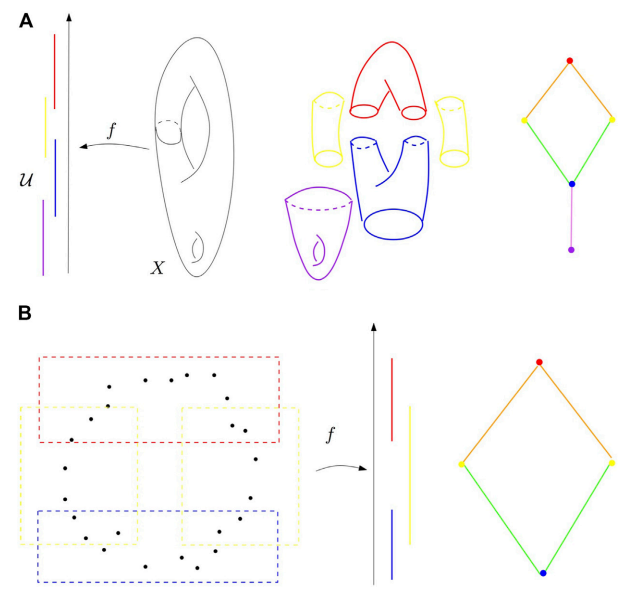
\includegraphics[width=0.85\linewidth]{./figures/Figura4.png}
    \caption{
        (A) Cubierta pull-back refinada de la funci\'on altura sobre una superficie en $\mathbb{R}^{3}$.
        (B) Algoritmo de Mapper en una nube de puntos muestreada alrededor de un c\'irculo y la
        funci\'on altura.
    }
    \label{fig:Figura 4}
    \vspace{15pt}
\end{figure}

\section*{La Elecci\'on de $f$}

La elecci\'on de la funci\'on $f$, a veces llamada la funci\'on filtro o lente, depende fuertemente de las
propiedades de los datos que uno pretende resaltar. Las siguientes son algunas de las m\'as encontradas en
la literatura:

\begin{itemize}
    \item Estimadores de densidad: El complejo Mapper puede ser \'util para entender la estructura y
    conexidad de \'areas de alta densidad.
    
    \item Coordenadas de an\'alisis de componentes principales (coordenadas PCA) o funciones coordenadas
    obtenidas de una t\'ecnica de reducci\'on de dimensionalidad no lineal (NLDR), eigenfunciones de
    laplacianos de gr\'aficas pueden ayudar a revelar y entender parte de la ambig\"uedad en el uso
    de reducciones de dimensionalidad no lineales.
    
    \item La funci\'on de centralidad $f\left(x\right) = \Sigma_{y\in\mathbb{X}}d\left(x,y\right)$ y la
    funci\'on de excentricidad $f\left(x\right) = \max_{y\in\mathbb{X}}d\left(x,y\right)$ a veces resultan
    ser buenas elecciones que no requieren de ning\'un conocimiento espec\'ifico acerca de los datos.
    
    \item Para datos muestreados sobre estructuras filamentarias de dimensi\'on uno, la funci\'on
    distancia a un punto dado permite recuperar la topolog\'ia subyacente de las estructuras filamentarias
    \cite{Chazal2015d}.
    
\end{itemize}

\section*{La Elecci\'on de la Cubierta $\mathcal{U}$}

Cuando $f$ es una funci\'on de valores reales, una elecci\'on est\'andar de $\mathcal{U}$
es un conjunto de intervalos espaciados regularmente y del mismo largo, $r>0$, cubriendo al conjunto
$f\left(\mathbb{X}\right)$. El n\'umero real $r$ es a veces llamado la resoluci\'on de
la cubierta, y el porcentaje $g$ de sobreposici\'on entre dos
intervalos consecutivos es llamado la ganancia de la cubierta.
N\'otese que si la ganancia $g$ es escogida menor a $50\%$, entonces cada punto de la linea real es
cubierto por, a lo m\'as, $2$ conjuntos abiertos de $\mathcal{U}$, y el nervio
resultante es una gr\'afica. Es importante notar que la salida de Mapper es muy
sensible a la elecci\'on de $\mathcal{U}$, y cambios
peque\~{n}os en la resoluci\'on o ganancia puede afectar de manera significativa al resultado, volviendo el
m\'etodo muy inestable. Una estrategia cl\'asica consiste en explorar un rango de par\'ametros y
seleccionar aquellos que sean m\'as informativos desde el punto de vista del usuario.

\section*{La Elecci\'on del Agrupamiento}

El algoritmo Mapper requiere el agrupamiento de la preimagen de conjuntos abiertos $U\in\mathcal{U}$.
Existen dos estrategias para realizar este agrupamiento. La primera consiste en aplicar, a cada
$U\in\mathcal{U}$, un algoritmo de agrupamiento, escogido por el usuario, a la preimagen de
$f^{-1}\left(U\right)$. La segunda, m\'as global, consiste en construir una gr\'afica sobre el
conjunto de datos $\mathbb{X}$, por ejemplo, una gr\'afica k-NN o una $\epsilon$-gr\'afica y, para cada
$U\in\mathcal{U}$, tomar las componentes conexas de la subgr\'afica con el conjunto de v\'ertices
$f^{-1}\left(U\right)$.

\section*{Aspectos Teor\'eticos y Estad\'isticos del Algoritmo Mapper}

Basados en los resultados de estabilidad y la estructura de Mapper propuestos en el estudio por
Carri\`ere y Oudot (2017) \cite{Carriere2017}, se han realizado avances en direcci\'on a
una versi\'on de Mapper estad\'isticamente bien fundamentada en el estudio por Carri\`ere et al. (2018)
\cite{Carriere2018}. De aqu\'i destaca que la convergencia de Mapper depende tanto del muestreo de los
datos como de la regularidad de la funci\'on filtro. M\'as aun, estrategias de submuestreo pueden ser
usadas para seleccionar un complejo en una filtraci\'on de Rips a una escala conveniente, as\'i como la
resoluci\'on y la ganancia para definir la gr\'afica Mapper. El caso para filtros estoc\'asticos y
multivariados tambi\'en ha sido estudiado por Carri\`ere y Michel (2019) \cite{Carriere2019}.
Una descripci\'on alternativa de la convergencia probabil\'istica de Mapper, en t\'erminos de la
categorificaci\'on, fue propuesta en el estudio por Brown et al. (2020) \cite{Brown2020}. Otros
acercamientos tambi\'en fueron propuestos para estudiar y lidiar con la inestabilidad del algoritmo
Mapper en los trabajos de Dey et al. (2016) \cite{Dey2016}, Dey et al. (2017) \cite{Dey2017}.

\section*{An\'alisis de Datos con Mapper}

Como una herramienta del an\'alisis de datos, Mapper se ha utilizado con \'exito para tareas de
agrupamiento y selecci\'on de atributos. La idea es identificar estructuras
espec\'ificas en la gr\'afica (o complejo) Mapper, en particular, lazos.
Estas estructuras son usadas para identificar
c\'umulos interesantes o seleccionar atributos que puedan diferenciar los datos en estas estructuras de
manera apropiada. Aplicaciones en datos reales ilustrando estas t\'ecnicas pueden ser encontradas en,
por ejemplo, los estudios por Carri\`ere y Rabad\'an (2020) \cite{Carriere2020}, Lum et al. (2013)
\cite{Lum2013}, Yao et al. (2009) \cite{Yao2009}.